Для создания карты глубины использовались фотографии, одна из которых приведенна на рисунке \ref{img:input_img}, а полученная карта приведена на рисунке \ref{img:result}.

\begin{figure}[h!]
	\center {
		\begin{minipage}{0.4\textwidth}
			\center {
				\includegraphics[width=\linewidth]{img/right2}
				\caption{Одно из изображений стереопары}\label{img:input_img}
			}
		\end{minipage}\hfill
		\begin{minipage}{0.4\textwidth}
			\center {
				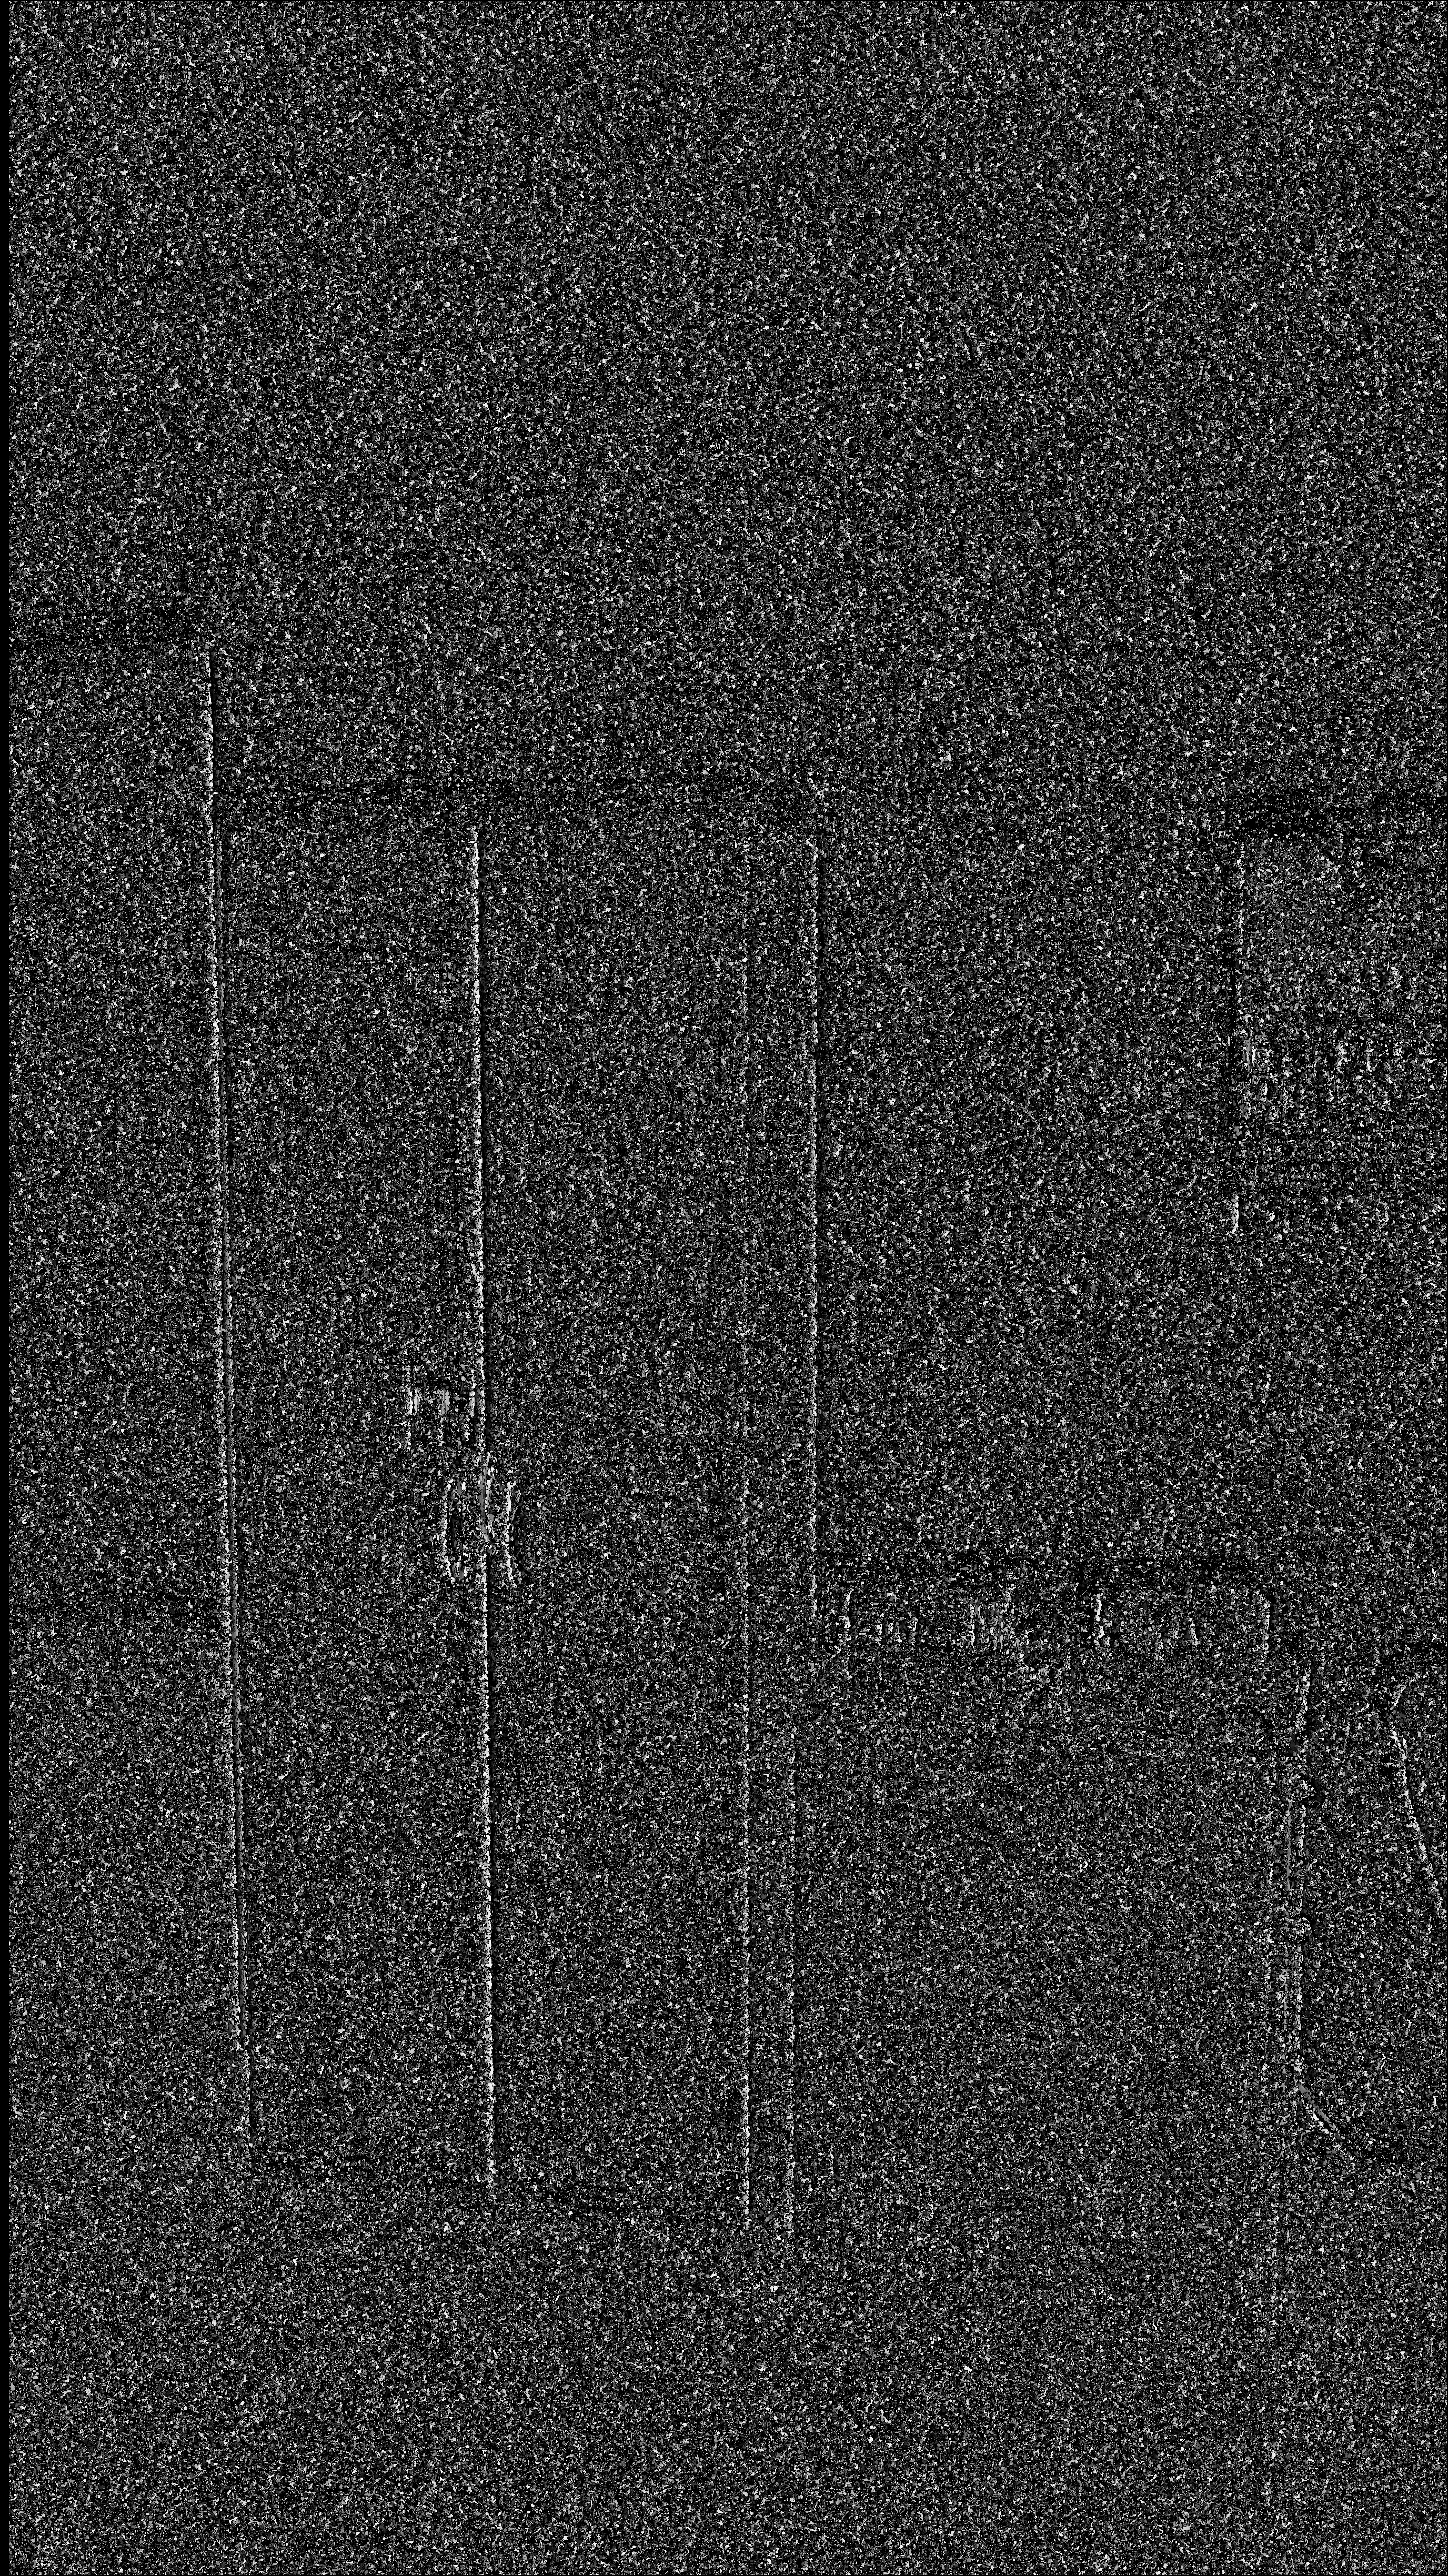
\includegraphics[width=\linewidth]{img/result}
				\caption{Полученная карта глубины}\label{img:result}
			}
		\end{minipage}\hfill
	}
\end{figure}